\page{5 / WATCH THE GAME}{What the moving technician really means}
Click the gearbox in \textbf{Factory Simulation}. Its inspector panel opens below the scene. Pressing \textbf{Send technician to inspect} submits an actual simulation action. The backend records the job and destination; the character walks to the component; the backend eventually records a completed observation. An accepted request is only the start of this sequence.

\begin{center}
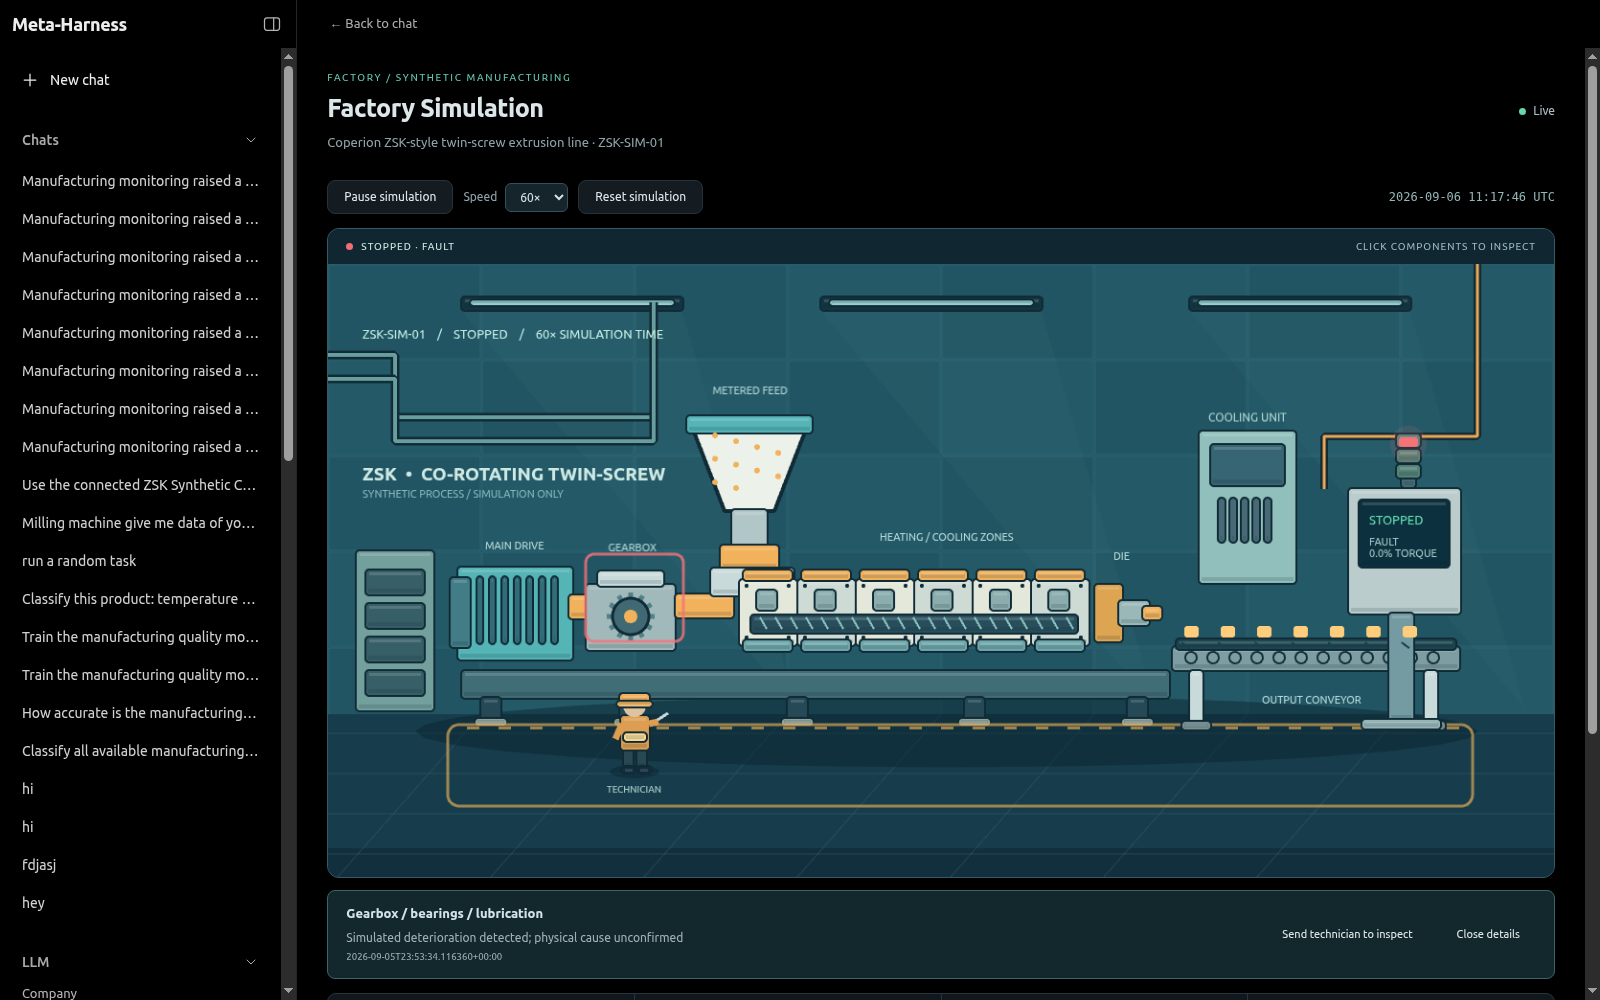
\includegraphics[width=\linewidth,trim=327bp 20bp 46bp 540bp,clip]{guide/figures/game-inspector.png}
\captionof{figure}{Saved game capture: technician at the gearbox, inspector open below the scene. The finding is synthetic deterioration, not a physical diagnosis. This is earlier verification evidence, not a new run.}
\end{center}

\subsection*{Read the scene without overreading it}
\begin{tabularx}{\linewidth}{@{}p{.30\linewidth}X@{}}\toprule
What you see & What the software actually does\\\midrule
Gears, screws and parcels move & Phaser draws generic motion from production mode and simulated time, not a calibrated physical model.\\
The technician walks or works & The backend owns position and job status. The browser smooths movement between snapshots.\\
A component flashes & The scene uses the alarm component, with a gearbox fallback before an alarm exists. Flashing alone is not diagnosis evidence.\\
An inspection finding appears & The backend checks injected scenarios for that component and returns a synthetic observation, not a mechanical test.\\\bottomrule
\end{tabularx}

\textbf{Pause simulation} freezes the simulated clock and pending actions. \textbf{Stop simulated line} stops production, but the clock can keep running so diagnostics finish. The backend runs even when the browser is closed. At 60×, ten simulated minutes take ten wall-clock seconds; the AI's response time is still real elapsed time.

\takeaway{The AI reads structured tool results, not the game image. The animation makes those results visible. Different faults mostly share the same machinery animation; the sensor records and inspection results distinguish them.}
\evidence{Rendering: \path{ui/src/components/factory/factory-scene.ts}. Clock, technician movement and inspection results: \path{factory-service/factory/domain.py}.}
